% Created 2019-05-17 Fri 15:58
% Intended LaTeX compiler: pdflatex
\documentclass[a4paper]{article}
\usepackage[utf8]{inputenc}
\usepackage[T1]{fontenc}
\usepackage{graphicx}
\usepackage{grffile}
\usepackage{longtable}
\usepackage{wrapfig}
\usepackage{rotating}
\usepackage[normalem]{ulem}
\usepackage{amsmath}
\usepackage{textcomp}
\usepackage{amssymb}
\usepackage{capt-of}
\usepackage{hyperref}
\usepackage{minted}
\usepackage[margin=0.8in]{geometry}
\usepackage{amssymb,amsmath}
\usepackage{fancyhdr}
\pagestyle{fancy}
\usepackage{lastpage}
\usepackage{float}
\restylefloat{figure}
\usepackage{hyperref}
\usepackage{tabularx}
\hypersetup{urlcolor=blue}
\usepackage{titlesec}
\setcounter{secnumdepth}{4}
\usepackage{minted}
\setminted{frame=single,framesep=10pt}
\chead{}
\rhead{\today}
\cfoot{}
\rfoot{\thepage\ of \pageref{LastPage}}
\usepackage[parfill]{parskip}
\usepackage{subfig}
\usepackage[sort&compress, numbers]{natbib}
\hypersetup{colorlinks=true,linkcolor=black, citecolor=black}
\usepackage{framed}
\usepackage{mathtools, cases}
\author{Nathan Hughes (JIC)}
\date{\today}
\title{RNA-seq Report}
\hypersetup{
 pdfauthor={Nathan Hughes (JIC)},
 pdftitle={RNA-seq Report},
 pdfkeywords={},
 pdfsubject={},
 pdfcreator={Emacs 26.1 (Org mode 9.1.9)},
 pdflang={English}}
\begin{document}

\maketitle
\maketitle
\clearpage
\tableofcontents
\clearpage


\section{Data setup}
\label{sec:orgcc69334}

\subsection{Helper funcs for pprinting}
\label{sec:org410a50a}

Lets go!


\subsection{Load up counts and DE}
\label{sec:org220b1be}
Loaded data

\clearpage
\subsection{Extracting gene names example}
\label{sec:orgce726bb}

\begin{center}
\begin{tabular}{rlll}
 & incoming & name & description\\
\hline
0 & AT1G73850 & AT1G73850 & Protein of unknown function (DUF1666)\\
1 & AT2G35210 & AGD10 & RPA\\
2 & AT5G23360 & AT5G23360 & GEM-like protein 7\\
3 & AT3G04480 & AT3G04480 & Endoribonuclease\\
4 & AT5G65165 & SDH2-3 & Succinate dehydrogenase\\
5 & AT2G08635 & AT2G08635 & None\\
6 & AT4G38810 & AT4G38810 & Calcium-binding EF-hand family protein\\
7 & AT3G63530 & BB & BB2\\
8 & AT2G33000 & AT2G33000 & Ubiquitin-associated (UBA)/TS-N domain-containing protein-like protein\\
9 & AT5G10336 & AT5G10336 & unknown protein\\
10 & AT3G21620 & AT3G21620 & CSC1-like protein At3g21620\\
11 & AT3G17225 & AT3G17225 & Plant invertase/pectin methylesterase inhibitor superfamily protein\\
12 & AT2G30910 & ARPC1A & Actin-related protein 2/3 complex subunit 1A\\
13 & AT5G50520 & AT5G50520 & Major facilitator superfamily protein\\
14 & AT5G19590 & AT5G19590 & At5g19590\\
15 & AT3G19190 & ATG2 & Autophagy-related protein 2\\
16 & AT5G01675 & AT5G01675 & None\\
17 & AT1G27040 & NPF4.5 & Protein NRT1/ PTR FAMILY 4.5\\
18 & AT3G49490 & AT3G49490 & Uncharacterized protein T9C5.90\\
19 & AT1G02890 & AT1G02890 & AAA-type ATPase family protein\\
\end{tabular}
\end{center}

\clearpage

\section{Inspect Samples}
\label{sec:orge2aba67}

\subsection{Creating a distance map of samples using normalised counts}
\label{sec:orgf6d54a1}


\subsubsection{Samples separated}
\label{sec:orgd88a24b}

\begin{verbatim}
<Figure size 720x720 with 4 Axes>
\end{verbatim}

\begin{figure}[htbp]
\centering
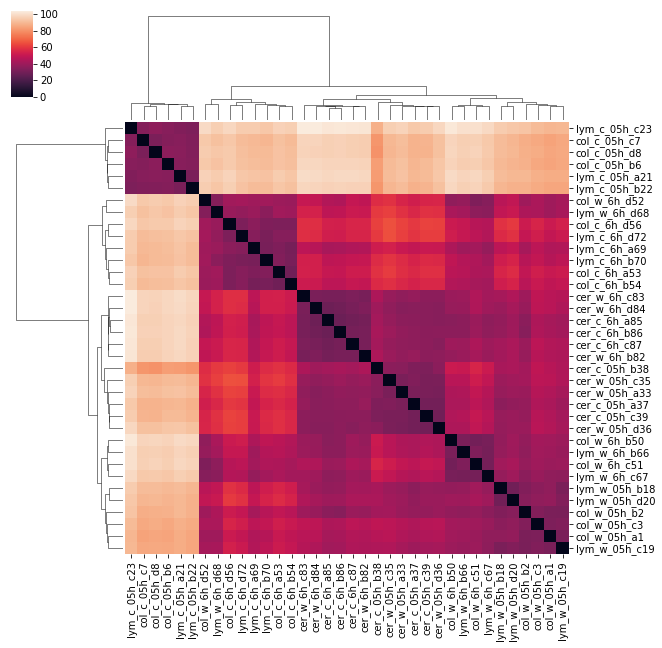
\includegraphics[width=.9\linewidth]{obipy-resources/distancemap.png}
\caption{\label{distancemap}
Distance map between samples}
\end{figure}

\subsubsection{Samples together}
\label{sec:org274e0c9}

\begin{verbatim}
<Figure size 720x720 with 5 Axes>
\end{verbatim}

\begin{figure}[htbp]
\centering
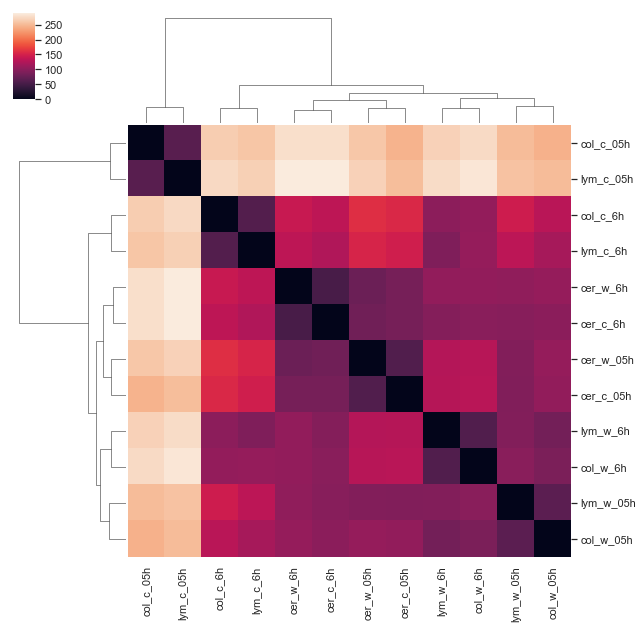
\includegraphics[width=15cm]{obipy-resources/distancemap_together.png}
\caption{\label{distancemappooled}
Distance map between samples, pooled together}
\end{figure}

\section{Simple Analysis}
\label{sec:org31c615b}

\subsection{Largest/Lowest expression sum}
\label{sec:orgcedbe0a}

\begin{verbatim}
<Figure size 720x720 with 4 Axes>
\end{verbatim}

\begin{figure}[htbp]
\centering
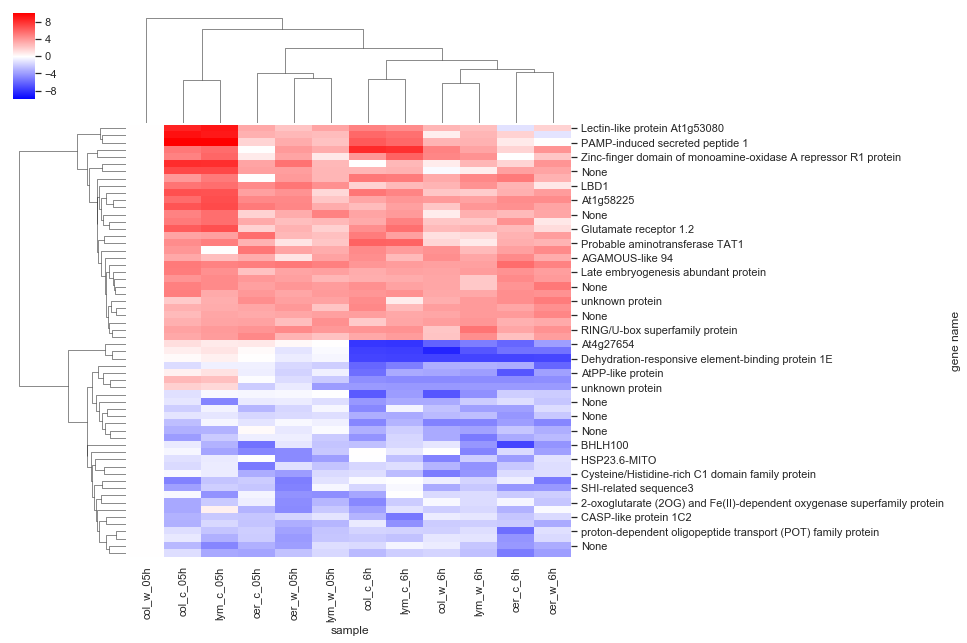
\includegraphics[width=15cm]{obipy-resources/large.png}
\caption{\label{largest}
Largest and least DE genes, values given are log2 fold changes /i.e a change of -1 is equivalent to \(2^{-1}\) or 0.5 the amount of control}
\end{figure}

\subsection{Largest/Lowest TF expression}
\label{sec:org6a47a65}

\begin{verbatim}
<Figure size 720x720 with 4 Axes>
\end{verbatim}

\begin{figure}[htbp]
\centering
\includegraphics[width=15cm]{obipy-resources/tfs.png}
\caption{\label{tfs}
Largest and least DE TFs, values given are log2 fold changes /i.e a change of -1 is equivalent to \(2^{-1}\) or 0.5 the amount of control}
\end{figure}



\subsection{Largest/Lowest deviation in log2foldchanges}
\label{sec:orgd8b7154}

\begin{verbatim}
<Figure size 720x720 with 4 Axes>
\end{verbatim}

\begin{figure}[htbp]
\centering
\includegraphics[width=15cm]{obipy-resources/deviation.png}
\caption{\label{largest}
Largest and least std DE genes, values given are log2 fold changes /i.e a change of -1 is equivalent to \(2^{-1}\) or 0.5 the amount of control}
\end{figure}

\subsection{PCA on count data}
\label{sec:orgb44efb5}

Explained varience from PC1 \& 2 respectively:
[0.54031803 0.14242627]

\begin{verbatim}
<Figure size 483.925x648 with 6 Axes>
\end{verbatim}

\begin{figure}[htbp]
\centering
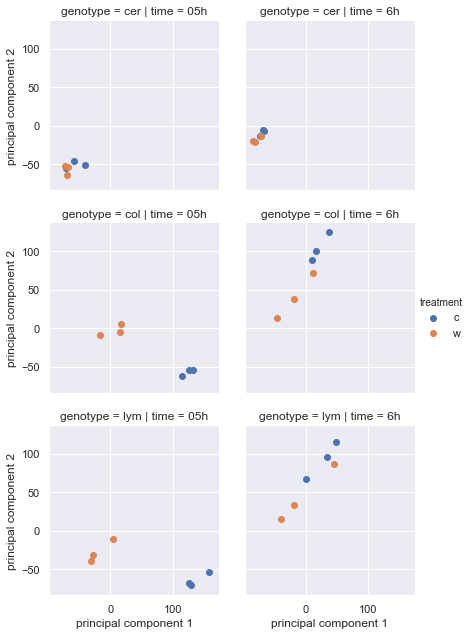
\includegraphics[width=15cm]{obipy-resources/pca.png}
\caption{\label{pca}
PCA of sample counts}
\end{figure}

\clearpage

\subsection{PCA on expression data}
\label{sec:org09358e9}

Explained varience from PC1 \& 2 respectively:
[0.77401765 0.14661658]

\begin{verbatim}
<Figure size 483.925x648 with 6 Axes>
\end{verbatim}

\begin{figure}[htbp]
\centering
\includegraphics[width=15cm]{obipy-resources/pca_minmax.png}
\caption{\label{pca_both}
PCA of sample min, max expression}
\end{figure}
\end{document}